\documentclass[10pt,a4paper]{amsart}
\usepackage[margin=19mm]{geometry}
\usepackage{amsmath,amssymb,mathtools}
\usepackage[scr=rsfs,cal=euler]{mathalfa}
\usepackage{xfrac}
\usepackage[unicode,hidelinks,bookmarks=false]{hyperref}
\newcommand{\ie}{i.e.\ }
\newcommand{\cf}{cf.\ }
\newcommand{\resp}{respectively\ }
\newcommand{\Subsection}{\subsection}
\providecommand{\nobreakdash}{\nobreak\hbox{-}}
\setlength{\emergencystretch}{2em}
\multlinegap0pt
\usepackage{tikz}
\usepackage{mathtools}
\usepackage{amssymb}
\usepackage{tensor}
\newtheorem{theorem}{Theorem}
\newtheorem{proposition}{Proposition}
\newcommand{\G}{\mathbb{G}}
\newcommand{\Hom}{\mathrm{Hom}}
\newcommand{\IM}{\mathrm{Im}}
\newcommand{\sym}{\mathrm{sym}}
\title{p-Primary Torsion of the Brauer Group in Characteristic p}
\author{Yuan Yang}
\date{Source: arXiv:2410.09969v3 (CC BY 4.0)}
\begin{document}
\maketitle

\noindent\emph{Source and licence.} p-Primary Torsion of the Brauer Group in Characteristic p. Version arXiv:2410.09969v3 (CC BY 4.0), distributed by arXiv under the Creative Commons Attribution 4.0 International licence, http://creativecommons.org/licenses/by/4.0/, as recorded in the arXiv licence metadata for this exact version and shown on the abstract page https://arxiv.org/abs/2410.09969v3. Full licence notice: \texttt{licenses/arxiv-2410.09969-CC-BY-4.0.txt}.\par\smallskip

\noindent\textit{Editorial scope.} Counted unit: the article's proposition HomGmnsym (source0.tex lines 2902--2904). The article's complete original proof of it is delivered with it (source0.tex lines 2906--3878, one \texttt{proof} environment of 973 lines). No mathematics is written, repaired or re-derived: the statement and the proof are the article's own lines, in the article's own notation, and no retained line is substituted or re-flowed.  Retained uncounted as the source-local context the proof needs: lines 2318--2324; lines 2373--2373.  Nothing was omitted from any retained span, so the package carries no omission record.  No retained line contains a citation, so the wrapper carries no bibliography and no bibliography entry.  The retained lines contain the article's own diagram code, which the wrapper typesets with the standard tikz packages; no image file is delivered and the package declares no asset dependency.  Editorial formatting only, in addition: an AMS \texttt{amsart} preamble that restates the article's own declarations and macros used by the retained lines, namely the environments \texttt{theorem}, \texttt{proposition} on separate counters, together with the standard packages those lines need.  The retained environments print in this document as Theorem 1, Proposition 1 in order of appearance, whereas the article prints the same items with the numbering of its own full document.  The complete native source of the article as distributed in the arXiv e-print for this exact version is bundled unchanged as \texttt{sources/166765/source0.tex}.
\begin{theorem} \label{E-O}
    Suppose $(A,\iota)$ is a principally polarized abelian variety of dimension $g$ 
    with Ekedahl-Oort type $\varphi=\varphi_P$, associated to a subset 
    $P=\{1\leqslant m_1<...<m_h\leqslant g\}$ of size $h$. 
    Then the dimension of $U[p]$ is given by: 
    \[\frac{(g-h)(g-h-1)}{2}+\sum_{i=1}^{h}(m_i-i).\]
\end{theorem}

\section{The Hom Group}\label{SectionTheHomGroup}

\begin{proposition}\label{HomGmnsym}
    The group \[\Hom(G_{m,n},G_{m,n}^\vee)^\sym\] has dimension $\frac{(m+n+1)(m+n)}{2}-\min\{m,n-1\}$.
\end{proposition}

\begin{proof}
    The covariant Dieudonné module of $G_{m,n}$ has the form: 
    \[e_1\xrightarrow{F}e_2\xleftarrow{V}e_3\xrightarrow{F}...\xleftarrow{V}e_{2m+1}\xrightarrow{F}e_{2m+2}\xrightarrow{F}e_{2m+3}\xleftarrow{V}...\xleftarrow{V}e_{2m+2n+2}\xleftarrow{V}e_1\]  
    The dual basis \(\{e_i^*\}\) then satisfies:
    \[e_1^*\xleftarrow{V}e_2^*\xrightarrow{F}e_3^*\xleftarrow{V}...\xrightarrow{F}e_{2m+1}^*\xleftarrow{V}e_{2m+2}^*\xleftarrow{V}e_{2m+3}^*\xrightarrow{F}...\xrightarrow{F}e_{2m+2n+2}^*\xrightarrow{F}e_1^*.\] 

    Let $x=\sum_{i=1}^{2m+2n+2}a_ie_i^*$, then a straightforward computation gives:
    \begin{equation}\label{GmnFV}
        \begin{aligned}
        F(x)&=a_{2m+2n+2}^\sigma e_1^*+\sum_{i=1}^m a_{2i}^\sigma e_{2i+1}^*+\sum_{i=m+2}^{m+n+1} a_{2i-1}^\sigma e_{2i}^*, \\
        V(x)&=\sum_{i=1}^{m+1} a_{2i}^{\sigma^{-1}}e_{2i-1}^*+\sum_{i=m+1}^{m+n} a_{2i+1}^{\sigma^{-1}}e_{2i}^*.
        \end{aligned}
    \end{equation}
    
    Let $f: G_{m,n}\rightarrow G_{m,n}^\vee$. 
    Following notations in Section \ref{SectionTheHomGroup}, 
    for $1\leqslant j\leqslant 2m+2n+2$, write 
    \[f(e_j)=\sum_{i=1}^{2m+2n+2} a_{i,j}e_i^*, \]

    We need to find the relations these coefficients $a_{i,j}$ need to satisfy. 
    These coefficients are given by a symmetric map $f: G_{m,n}\rightarrow G_{m,n}^\vee$ 
    if and only if they satisfy the following conditions: 
    \begin{itemize}
        \item For \(j=1,...,m\), we have \(F(f(e_{2j-1}))=f(e_{2j})=V(f(e_{2j+1})).\) 
        \item \(F(F(f(e_{2m+1})))=F(f(e_{2m+2}))=f(e_{2m+3})=V(f(e_{2m+4})).\)
        \item For \(j=m+2,...,m+n-1\), we have \(F(f(e_{2j}))=f(e_{2j+1})=V(f(e_{2j+2}))\).
        \item \(F(f(e_{2m+2n}))=f(e_{2m+2n+1})=V(f(e_{2m+2n+2}))=V(V(f(e_1)))\). 
        \item The matrix $[f]$ formed by $\{a_{i,j}\}$ is anti-symmetric.
    \end{itemize}

    Just as the proof of \ref{E-O}, we draw a direct graph that encodes all the combinatorial conditions. 
    We draw a $(2m+2n+2)\times(2m+2n+2)$ 
    grid with $a_{i,j}$ in the $i$-th row and $j$-th column. 
    An arrow from $a_{i_1,j_1}$ to $a_{i_2,j_2}$ indicates that
    that $a_{i_2,j_2}=a_{i_1,j_1}^\sigma$ is required in the Dieudonn\'e relations. 
    (Unlike in the previous section, here we take the target to be the Frobenius of the source for convenience.)
    An entry $a_{i,j}$ is marked $0$ if and only if $a_{i,j}=0$ 
    is required in the Dieudonné relations. 

    Define: \[P:= \{2j|k=1,2,...,m+1\}\cup \{2j+1|j=m+1,...,m+n\},\]
    \[Q:=\{2j|k=1,2,...,m\}\cup \{2j+1|j=m+1,...,m+n\}\cup \{2m+2n+2\}.\]

    Then: 
    \begin{itemize}
        \item $\{e_i|i\in P\}$ spans $\IM{(F)}$ of the covariant Dieudonné module of $G_{m,n}$. 
        \item $\{e_i^*|i \notin P\}$ spans $\IM{F}$ of the covariant Dieudonné module of $G_{m,n}^\vee$. 
        \item $\{e_i|i\in Q\}$ spans $\IM{(V)}$ of the covariant Dieudonné module of $G_{m,n}$. 
        \item $\{e_i^*|i \notin Q\}$ spans $\IM{(V)}$ of the covariant Dieudonné module of $G_{m,n}^\vee$. 
    \end{itemize}
    We have \[\#P=\#Q=m+n+1, \#(P\cap Q)=m+n.\]
   
The Dieudonné module structure and the symmetry conditions then imply:  
\begin{itemize}
    \item All diagonal entries vanish, since we require the matrix to be anti-symmetric. 
    \item Each arrow indicates that the target equals the Frobenius of the source.
    \item For any $j\in P$, since $f(e_j)=F(f(e_{j-1}))$, formula \ref{GmnFV} forces: for any $i\in P$, $a_{i,j}=0$; 
    for any $i \notin P$, we draw an arrow from $a_{i-1,j-1}$ to $a_{i,j}$. 
    \item For any $j\in Q$, since $f(e_j)=V(f(e_{j+1}))$, formula \ref{GmnFV} forces: for any $i\in Q$, $a_{i,j}=0$;
    for each $i\notin Q$, we draw an arrow from $a_{ij}$ to $a_{i+1,j+1}$. 
    \item The matrix has to be anti-symmetric. 
\end{itemize}

    Let us first settle the case $n-1\leqslant m$. 
    We take $m=4$ and $n=3$ to illustrate. 
    We show that: in this case, under the above conditions, there are exactly
    \[\frac{(m+1)m}{2}+(m+1)(n-1)+(m+1)+\frac{(n-1)(n-2)}{2}=\frac{(m+n+1)(m+n)}{2}-(n-1)\]
    degrees of freedom for the coefficients $\{a_{i,j}\}$.


    \begin{center}
        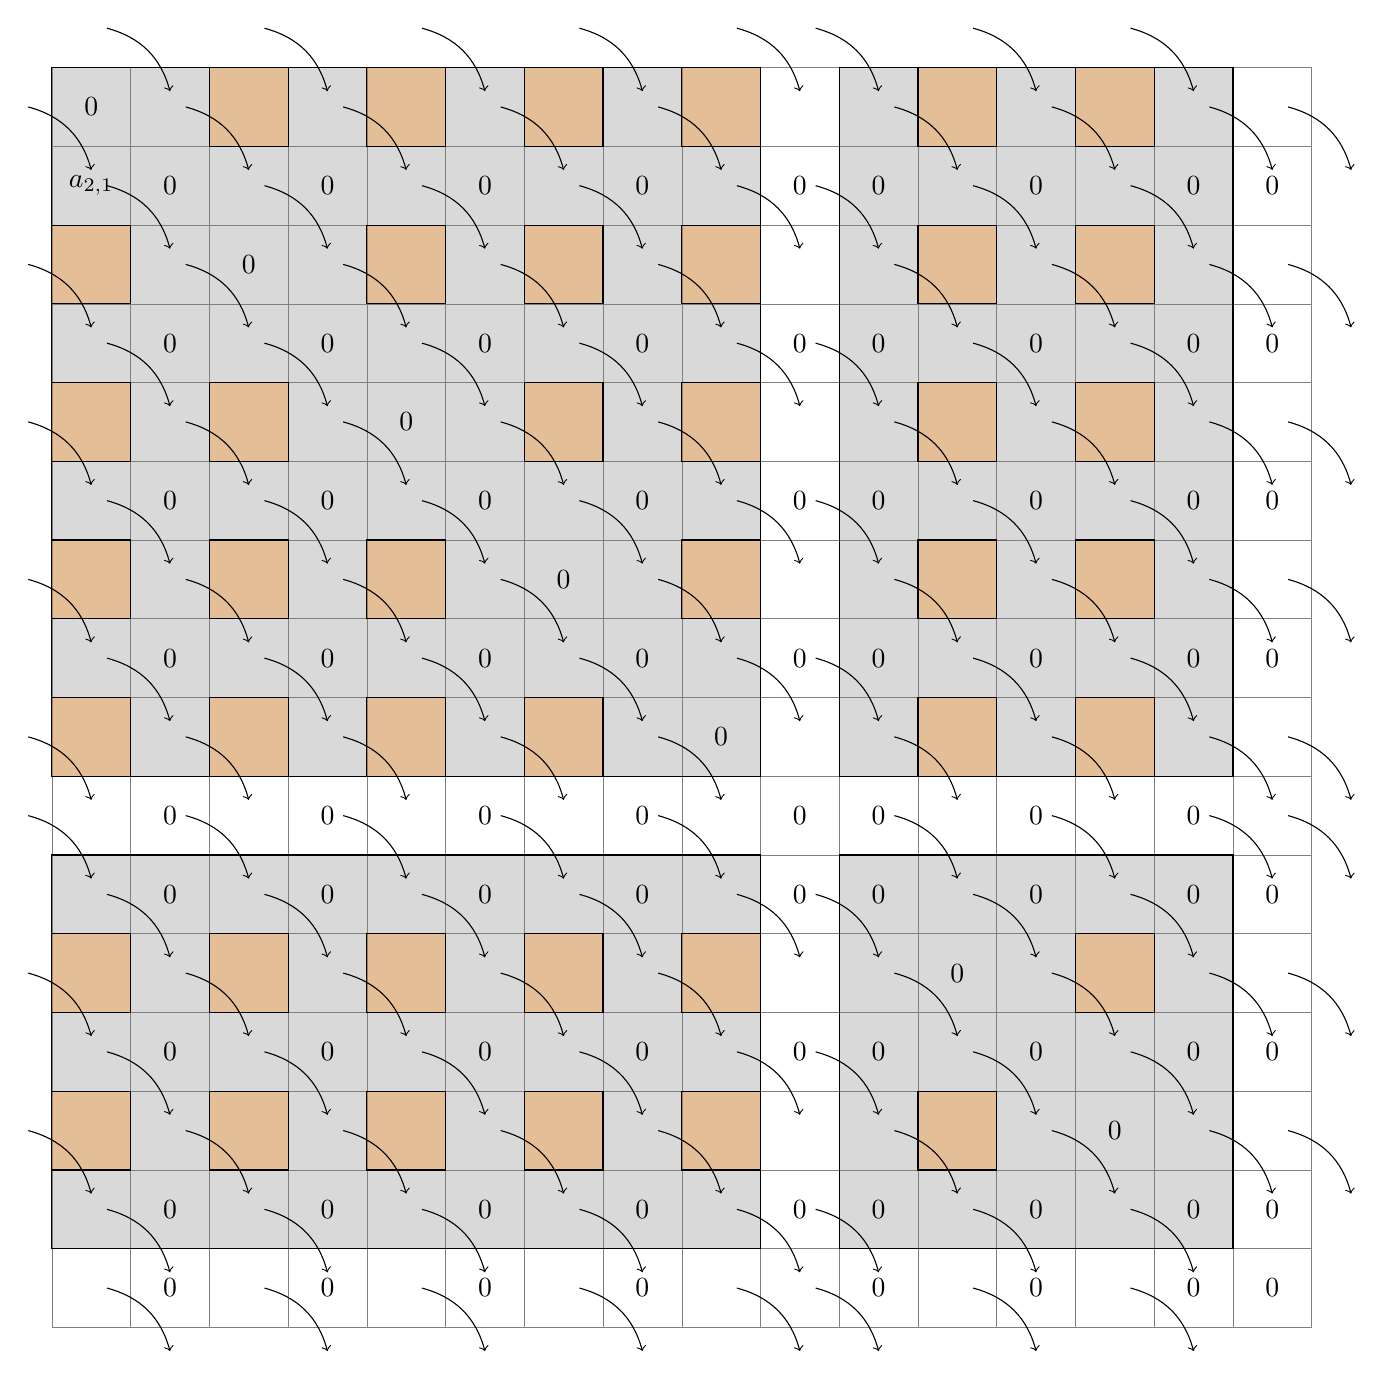
\begin{tikzpicture}
            \draw [step=1cm,gray,very thin] (0,0) grid (16,16);
            \filldraw[fill=gray, fill opacity=0.3, draw=black] (0,7) rectangle (9,16);
            \filldraw[fill=gray, fill opacity=0.3, draw=black] (10,1) rectangle (15,6);
            \filldraw[fill=gray, fill opacity=0.3, draw=black] (0,1) rectangle (9,6);
            \filldraw[fill=gray, fill opacity=0.3, draw=black] (10,7) rectangle (15,16);
            \node at (0.5,15.5){0};
            \node at (1.5,14.5){0};
            \node at (1.5,12.5){0};
            \node at (1.5,10.5){0};
            \node at (1.5,8.5){0};
            \node at (1.5,6.5){0};
            \node at (1.5,5.5){0};
            \node at (1.5,3.5){0};
            \node at (1.5,1.5){0};
            \node at (1.5,0.5){0};
            \node at (3.5,14.5){0};
            \node at (3.5,12.5){0};
            \node at (3.5,10.5){0};
            \node at (3.5,8.5){0};
            \node at (3.5,6.5){0};
            \node at (3.5,5.5){0};
            \node at (3.5,3.5){0};
            \node at (3.5,1.5){0};
            \node at (3.5,0.5){0};
            \node at (5.5,14.5){0};
            \node at (5.5,12.5){0};
            \node at (5.5,10.5){0};
            \node at (5.5,8.5){0};
            \node at (5.5,6.5){0};
            \node at (5.5,5.5){0};
            \node at (5.5,3.5){0};
            \node at (5.5,1.5){0};
            \node at (5.5,0.5){0};
            \node at (7.5,14.5){0};
            \node at (7.5,12.5){0};
            \node at (7.5,10.5){0};
            \node at (7.5,8.5){0};
            \node at (7.5,6.5){0};
            \node at (7.5,5.5){0};
            \node at (7.5,3.5){0};
            \node at (7.5,1.5){0};
            \node at (7.5,0.5){0};
            \node at (9.5,14.5){0};
            \node at (9.5,12.5){0};
            \node at (9.5,10.5){0};
            \node at (9.5,8.5){0};
            \node at (9.5,6.5){0};
            \node at (9.5,5.5){0};
            \node at (9.5,3.5){0};
            \node at (9.5,1.5){0};
            \node at (10.5,14.5){0};
            \node at (10.5,12.5){0};
            \node at (10.5,10.5){0};
            \node at (10.5,8.5){0};
            \node at (10.5,6.5){0};
            \node at (10.5,5.5){0};
            \node at (10.5,3.5){0};
            \node at (10.5,1.5){0};
            \node at (10.5,0.5){0};
            \node at (12.5,14.5){0};
            \node at (12.5,12.5){0};
            \node at (12.5,10.5){0};
            \node at (12.5,8.5){0};
            \node at (12.5,6.5){0};
            \node at (12.5,5.5){0};
            \node at (12.5,3.5){0};
            \node at (12.5,1.5){0};
            \node at (12.5,0.5){0};
            \node at (14.5,14.5){0};
            \node at (14.5,12.5){0};
            \node at (14.5,10.5){0};
            \node at (14.5,8.5){0};
            \node at (14.5,6.5){0};
            \node at (14.5,5.5){0};
            \node at (14.5,3.5){0};
            \node at (14.5,1.5){0};
            \node at (14.5,0.5){0};
            \node at (15.5,14.5){0};
            \node at (15.5,12.5){0};
            \node at (15.5,10.5){0};
            \node at (15.5,8.5){0};
            \node at (15.5,5.5){0};
            \node at (15.5,3.5){0};
            \node at (15.5,1.5){0};
            \node at (15.5,0.5){0};

            \node at (2.5,13.5){0};
            \node at (4.5,11.5){0};
            \node at (6.5,9.5){0};
            \node at (8.5,7.5){0};
            \node at (11.5,4.5){0};
            \node at (13.5,2.5){0};

            \filldraw[fill=orange, fill opacity=0.3, draw=black] (0,13) rectangle (1,14);
            \filldraw[fill=orange, fill opacity=0.3, draw=black] (0,11) rectangle (1,12);
            \filldraw[fill=orange, fill opacity=0.3, draw=black] (0,9) rectangle (1,10);
            \filldraw[fill=orange, fill opacity=0.3, draw=black] (0,7) rectangle (1,8);

            \filldraw[fill=orange, fill opacity=0.3, draw=black] (2,11) rectangle (3,12);
            \filldraw[fill=orange, fill opacity=0.3, draw=black] (2,9) rectangle (3,10);
            \filldraw[fill=orange, fill opacity=0.3, draw=black] (2,7) rectangle (3,8);

            \filldraw[fill=orange, fill opacity=0.3, draw=black] (4,9) rectangle (5,10);
            \filldraw[fill=orange, fill opacity=0.3, draw=black] (4,7) rectangle (5,8);

            \filldraw[fill=orange, fill opacity=0.3, draw=black] (6,7) rectangle (7,8);

            \filldraw[fill=orange, fill opacity=0.3, draw=black] (2,15) rectangle (3,16);
            \filldraw[fill=orange, fill opacity=0.3, draw=black] (4,15) rectangle (5,16);
            \filldraw[fill=orange, fill opacity=0.3, draw=black] (6,15) rectangle (7,16);
            \filldraw[fill=orange, fill opacity=0.3, draw=black] (8,15) rectangle (9,16);

            \filldraw[fill=orange, fill opacity=0.3, draw=black] (4,13) rectangle (5,14);
            \filldraw[fill=orange, fill opacity=0.3, draw=black] (6,13) rectangle (7,14);
            \filldraw[fill=orange, fill opacity=0.3, draw=black] (8,13) rectangle (9,14);

            \filldraw[fill=orange, fill opacity=0.3, draw=black] (6,11) rectangle (7,12);
            \filldraw[fill=orange, fill opacity=0.3, draw=black] (8,11) rectangle (9,12);

            \filldraw[fill=orange, fill opacity=0.3, draw=black] (8,9) rectangle (9,10);

            \filldraw[fill=orange, fill opacity=0.3, draw=black] (0,2) rectangle (1,3);
            \filldraw[fill=orange, fill opacity=0.3, draw=black] (2,2) rectangle (3,3);
            \filldraw[fill=orange, fill opacity=0.3, draw=black] (4,2) rectangle (5,3);
            \filldraw[fill=orange, fill opacity=0.3, draw=black] (6,2) rectangle (7,3);
            \filldraw[fill=orange, fill opacity=0.3, draw=black] (8,2) rectangle (9,3);

            \filldraw[fill=orange, fill opacity=0.3, draw=black] (0,4) rectangle (1,5);
            \filldraw[fill=orange, fill opacity=0.3, draw=black] (2,4) rectangle (3,5);
            \filldraw[fill=orange, fill opacity=0.3, draw=black] (4,4) rectangle (5,5);
            \filldraw[fill=orange, fill opacity=0.3, draw=black] (6,4) rectangle (7,5);
            \filldraw[fill=orange, fill opacity=0.3, draw=black] (8,4) rectangle (9,5);

            \filldraw[fill=orange, fill opacity=0.3, draw=black] (11,7) rectangle (12,8);
            \filldraw[fill=orange, fill opacity=0.3, draw=black] (11,9) rectangle (12,10);
            \filldraw[fill=orange, fill opacity=0.3, draw=black] (11,11) rectangle (12,12);
            \filldraw[fill=orange, fill opacity=0.3, draw=black] (11,13) rectangle (12,14);
            \filldraw[fill=orange, fill opacity=0.3, draw=black] (11,15) rectangle (12,16);

            \filldraw[fill=orange, fill opacity=0.3, draw=black] (13,7) rectangle (14,8);
            \filldraw[fill=orange, fill opacity=0.3, draw=black] (13,9) rectangle (14,10);
            \filldraw[fill=orange, fill opacity=0.3, draw=black] (13,11) rectangle (14,12);
            \filldraw[fill=orange, fill opacity=0.3, draw=black] (13,13) rectangle (14,14);
            \filldraw[fill=orange, fill opacity=0.3, draw=black] (13,15) rectangle (14,16);

            
            \filldraw[fill=orange, fill opacity=0.3, draw=black] (11,2) rectangle (12,3);
            
            \filldraw[fill=orange, fill opacity=0.3, draw=black] (13,4) rectangle (14,5);

            \draw[->] (-0.3,15.5) to[bend left] (0.5,14.7);
            \draw[->] (-0.3,13.5) to[bend left] (0.5,12.7);
            \draw[->] (-0.3,11.5) to[bend left] (0.5,10.7);
            \draw[->] (-0.3,9.5) to[bend left] (0.5,8.7);
            \draw[->] (-0.3,7.5) to[bend left] (0.5,6.7);
            \draw[->] (-0.3,6.5) to[bend left] (0.5,5.7);
            \draw[->] (-0.3,4.5) to[bend left] (0.5,3.7);
            \draw[->] (-0.3,2.5) to[bend left] (0.5,1.7);

            \draw[->] (0.7,16.5) to[bend left] (1.5,15.7);
            \draw[->] (0.7,14.5) to[bend left] (1.5,13.7);
            \draw[->] (0.7,12.5) to[bend left] (1.5,11.7);
            \draw[->] (0.7,10.5) to[bend left] (1.5,9.7);
            \draw[->] (0.7,8.5) to[bend left] (1.5,7.7);
            \draw[->] (0.7,5.5) to[bend left] (1.5,4.7);
            \draw[->] (0.7,3.5) to[bend left] (1.5,2.7);
            \draw[->] (0.7,1.5) to[bend left] (1.5,0.7);
            \draw[->] (0.7,0.5) to[bend left] (1.5,-0.3);

            \draw[->] (1.7,15.5) to[bend left] (2.5,14.7);
            \draw[->] (1.7,13.5) to[bend left] (2.5,12.7);
            \draw[->] (1.7,11.5) to[bend left] (2.5,10.7);
            \draw[->] (1.7,9.5) to[bend left] (2.5,8.7);
            \draw[->] (1.7,7.5) to[bend left] (2.5,6.7);
            \draw[->] (1.7,6.5) to[bend left] (2.5,5.7);
            \draw[->] (1.7,4.5) to[bend left] (2.5,3.7);
            \draw[->] (1.7,2.5) to[bend left] (2.5,1.7);

            \draw[->] (2.7,16.5) to[bend left] (3.5,15.7);
            \draw[->] (2.7,14.5) to[bend left] (3.5,13.7);
            \draw[->] (2.7,12.5) to[bend left] (3.5,11.7);
            \draw[->] (2.7,10.5) to[bend left] (3.5,9.7);
            \draw[->] (2.7,8.5) to[bend left] (3.5,7.7);
            \draw[->] (2.7,5.5) to[bend left] (3.5,4.7);
            \draw[->] (2.7,3.5) to[bend left] (3.5,2.7);
            \draw[->] (2.7,1.5) to[bend left] (3.5,0.7);
            \draw[->] (2.7,0.5) to[bend left] (3.5,-0.3);

            \draw[->] (3.7,15.5) to[bend left] (4.5,14.7);
            \draw[->] (3.7,13.5) to[bend left] (4.5,12.7);
            \draw[->] (3.7,11.5) to[bend left] (4.5,10.7);
            \draw[->] (3.7,9.5) to[bend left] (4.5,8.7);
            \draw[->] (3.7,7.5) to[bend left] (4.5,6.7);
            \draw[->] (3.7,6.5) to[bend left] (4.5,5.7);
            \draw[->] (3.7,4.5) to[bend left] (4.5,3.7);
            \draw[->] (3.7,2.5) to[bend left] (4.5,1.7);

            \draw[->] (4.7,16.5) to[bend left] (5.5,15.7);
            \draw[->] (4.7,14.5) to[bend left] (5.5,13.7);
            \draw[->] (4.7,12.5) to[bend left] (5.5,11.7);
            \draw[->] (4.7,10.5) to[bend left] (5.5,9.7);
            \draw[->] (4.7,8.5) to[bend left] (5.5,7.7);
            \draw[->] (4.7,5.5) to[bend left] (5.5,4.7);
            \draw[->] (4.7,3.5) to[bend left] (5.5,2.7);
            \draw[->] (4.7,1.5) to[bend left] (5.5,0.7);
            \draw[->] (4.7,0.5) to[bend left] (5.5,-0.3);

            \draw[->] (5.7,15.5) to[bend left] (6.5,14.7);
            \draw[->] (5.7,13.5) to[bend left] (6.5,12.7);
            \draw[->] (5.7,11.5) to[bend left] (6.5,10.7);
            \draw[->] (5.7,9.5) to[bend left] (6.5,8.7);
            \draw[->] (5.7,7.5) to[bend left] (6.5,6.7);
            \draw[->] (5.7,6.5) to[bend left] (6.5,5.7);
            \draw[->] (5.7,4.5) to[bend left] (6.5,3.7);
            \draw[->] (5.7,2.5) to[bend left] (6.5,1.7);

            \draw[->] (6.7,16.5) to[bend left] (7.5,15.7);
            \draw[->] (6.7,14.5) to[bend left] (7.5,13.7);
            \draw[->] (6.7,12.5) to[bend left] (7.5,11.7);
            \draw[->] (6.7,10.5) to[bend left] (7.5,9.7);
            \draw[->] (6.7,8.5) to[bend left] (7.5,7.7);
            \draw[->] (6.7,5.5) to[bend left] (7.5,4.7);
            \draw[->] (6.7,3.5) to[bend left] (7.5,2.7);
            \draw[->] (6.7,1.5) to[bend left] (7.5,0.7);
            \draw[->] (6.7,0.5) to[bend left] (7.5,-0.3);

            \draw[->] (7.7,15.5) to[bend left] (8.5,14.7);
            \draw[->] (7.7,13.5) to[bend left] (8.5,12.7);
            \draw[->] (7.7,11.5) to[bend left] (8.5,10.7);
            \draw[->] (7.7,9.5) to[bend left] (8.5,8.7);
            \draw[->] (7.7,7.5) to[bend left] (8.5,6.7);
            \draw[->] (7.7,6.5) to[bend left] (8.5,5.7);
            \draw[->] (7.7,4.5) to[bend left] (8.5,3.7);
            \draw[->] (7.7,2.5) to[bend left] (8.5,1.7);

            \draw[->] (8.7,16.5) to[bend left] (9.5,15.7);
            \draw[->] (8.7,14.5) to[bend left] (9.5,13.7);
            \draw[->] (8.7,12.5) to[bend left] (9.5,11.7);
            \draw[->] (8.7,10.5) to[bend left] (9.5,9.7);
            \draw[->] (8.7,8.5) to[bend left] (9.5,7.7);
            \draw[->] (8.7,5.5) to[bend left] (9.5,4.7);
            \draw[->] (8.7,3.5) to[bend left] (9.5,2.7);
            \draw[->] (8.7,1.5) to[bend left] (9.5,0.7);
            \draw[->] (8.7,0.5) to[bend left] (9.5,-0.3);

            \draw[->] (9.7,16.5) to[bend left] (10.5,15.7);
            \draw[->] (9.7,14.5) to[bend left] (10.5,13.7);
            \draw[->] (9.7,12.5) to[bend left] (10.5,11.7);
            \draw[->] (9.7,10.5) to[bend left] (10.5,9.7);
            \draw[->] (9.7,8.5) to[bend left] (10.5,7.7);
            \draw[->] (9.7,5.5) to[bend left] (10.5,4.7);
            \draw[->] (9.7,3.5) to[bend left] (10.5,2.7);
            \draw[->] (9.7,1.5) to[bend left] (10.5,0.7);
            \draw[->] (9.7,0.5) to[bend left] (10.5,-0.3);

            \draw[->] (10.7,15.5) to[bend left] (11.5,14.7);
            \draw[->] (10.7,13.5) to[bend left] (11.5,12.7);
            \draw[->] (10.7,11.5) to[bend left] (11.5,10.7);
            \draw[->] (10.7,9.5) to[bend left] (11.5,8.7);
            \draw[->] (10.7,7.5) to[bend left] (11.5,6.7);
            \draw[->] (10.7,6.5) to[bend left] (11.5,5.7);
            \draw[->] (10.7,4.5) to[bend left] (11.5,3.7);
            \draw[->] (10.7,2.5) to[bend left] (11.5,1.7);

            \draw[->] (11.7,16.5) to[bend left] (12.5,15.7);
            \draw[->] (11.7,14.5) to[bend left] (12.5,13.7);
            \draw[->] (11.7,12.5) to[bend left] (12.5,11.7);
            \draw[->] (11.7,10.5) to[bend left] (12.5,9.7);
            \draw[->] (11.7,8.5) to[bend left] (12.5,7.7);
            \draw[->] (11.7,5.5) to[bend left] (12.5,4.7);
            \draw[->] (11.7,3.5) to[bend left] (12.5,2.7);
            \draw[->] (11.7,1.5) to[bend left] (12.5,0.7);
            \draw[->] (11.7,0.5) to[bend left] (12.5,-0.3);

            \draw[->] (12.7,15.5) to[bend left] (13.5,14.7);
            \draw[->] (12.7,13.5) to[bend left] (13.5,12.7);
            \draw[->] (12.7,11.5) to[bend left] (13.5,10.7);
            \draw[->] (12.7,9.5) to[bend left] (13.5,8.7);
            \draw[->] (12.7,7.5) to[bend left] (13.5,6.7);
            \draw[->] (12.7,6.5) to[bend left] (13.5,5.7);
            \draw[->] (12.7,4.5) to[bend left] (13.5,3.7);
            \draw[->] (12.7,2.5) to[bend left] (13.5,1.7);

            \draw[->] (13.7,16.5) to[bend left] (14.5,15.7);
            \draw[->] (13.7,14.5) to[bend left] (14.5,13.7);
            \draw[->] (13.7,12.5) to[bend left] (14.5,11.7);
            \draw[->] (13.7,10.5) to[bend left] (14.5,9.7);
            \draw[->] (13.7,8.5) to[bend left] (14.5,7.7);
            \draw[->] (13.7,5.5) to[bend left] (14.5,4.7);
            \draw[->] (13.7,3.5) to[bend left] (14.5,2.7);
            \draw[->] (13.7,1.5) to[bend left] (14.5,0.7);
            \draw[->] (13.7,0.5) to[bend left] (14.5,-0.3);

            \draw[->] (14.7,15.5) to[bend left] (15.5,14.7);
            \draw[->] (14.7,13.5) to[bend left] (15.5,12.7);
            \draw[->] (14.7,11.5) to[bend left] (15.5,10.7);
            \draw[->] (14.7,9.5) to[bend left] (15.5,8.7);
            \draw[->] (14.7,7.5) to[bend left] (15.5,6.7);
            \draw[->] (14.7,6.5) to[bend left] (15.5,5.7);
            \draw[->] (14.7,4.5) to[bend left] (15.5,3.7);
            \draw[->] (14.7,2.5) to[bend left] (15.5,1.7);

            \draw[->] (15.7,15.5) to[bend left] (16.5,14.7);
            \draw[->] (15.7,13.5) to[bend left] (16.5,12.7);
            \draw[->] (15.7,11.5) to[bend left] (16.5,10.7);
            \draw[->] (15.7,9.5) to[bend left] (16.5,8.7);
            \draw[->] (15.7,7.5) to[bend left] (16.5,6.7);
            \draw[->] (15.7,6.5) to[bend left] (16.5,5.7);
            \draw[->] (15.7,4.5) to[bend left] (16.5,3.7);
            \draw[->] (15.7,2.5) to[bend left] (16.5,1.7);

            \node at (0.5,14.5){$a_{2,1}$};
        \end{tikzpicture}
    \end{center}

    To understand the relations and the $0$'s in this grid, 
    we consider the following four different regions (the gray areas in the picture): 
    \begin{itemize}
        \item $S_1$, entries $a_{ij}$ such that $1\leqslant i,j\leqslant 2m+1$;
        \item  $S_2$, entries $a_{ij}$ such that $2m+3\leqslant i\leqslant 2m+2n+1, \quad 1\leqslant j\leqslant 2m+1$;
        \item  $S_3$, entries $a_{ij}$ such that $1\leqslant i\leqslant 2m+1, \quad 2m+3\leqslant j\leqslant 2m+2n+1$;
        \item  $S_4$, entries $a_{ij}$ such that $ 2m+3\leqslant i,j\leqslant 2m+2n+1$.
    \end{itemize}

    
    Within these regions, some coefficients have neither a marked $0$, nor any incoming or outgoing arrows. 
    We mark these coefficients with orange boxes. 
    They represent variables with no constraints. 
    There are exactly \[\frac{m(m+1)}{2}+(m+1)(n-1)+\frac{(n-1)(n-2)}{2}\] pairs (under symmetric along the diagonal) of such boxes. 

    When $m>n-1$, there are exactly $m+1$ symmetric pairs of free orbits, 
    namely those passing though $a_{2i,1}$, for $i=1,2,...,m+1$. 
    All other orbits, either start or end at a $0$. 
    Each pair of free orbits corresponds to one copy of $\G_a$.
    Counting the total dimension, we have exactly
    \[\frac{(m+1)m}{2}+(m+1)(n-1)+\frac{(n-1)(n-2)}{2}+(m+1)=\frac{(m+n+1)(m+n)}{2}-(n-1)\]
    degrees of freedom under the symmetric condition and the Dieudonn\'e conditions. 
    
    When $m=n-1$, we illustrate the picture with the example $m=2$, $n=3$. 
    We again find exactly $m+1$ pairs of free orbits, 
    those passing though $a_{2i,1}$, for $i=1,2,...,m+1$.
    In addition, there is one extra orbit (passing through $a_{2m+2,1}$)forming a cycle, 
    which does not contribute to unipotent dimension. 
    The same counting formula applies, giving 
    \[\frac{(m+1)m}{2}+(m+1)(n-1)+\frac{(n-1)(n-2)}{2}+(m+1)=\frac{(m+n+1)(m+n)}{2}-(n-1)\]
    degrees of freedom on the variables under the symmetric condition and the Dieudonn\'e conditions. 
    
    \begin{center}
        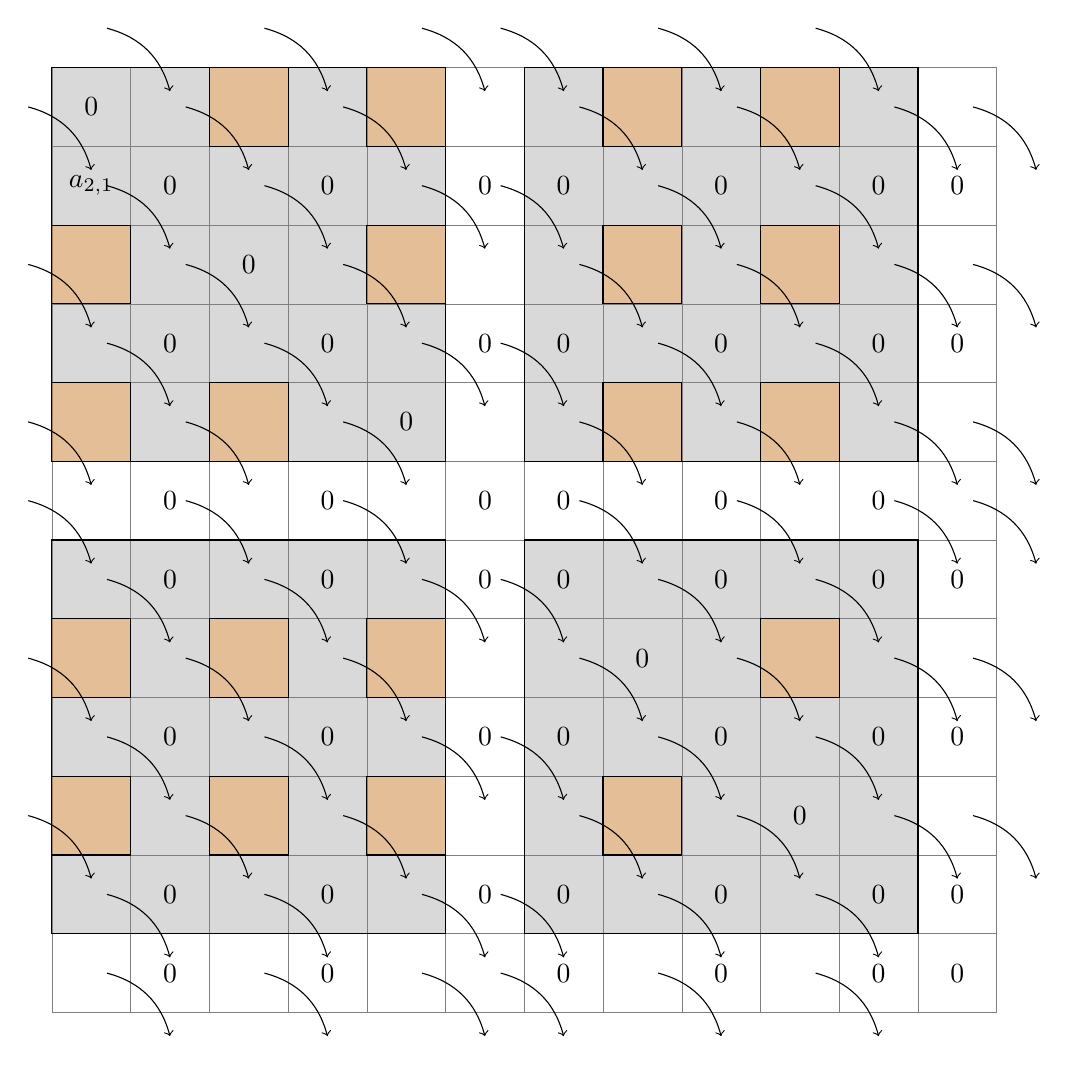
\begin{tikzpicture}
            \draw [step=1cm,gray,very thin] (0,0) grid (12,12);
            \filldraw[fill=gray, fill opacity=0.3, draw=black] (0,7) rectangle (5,12);
            \filldraw[fill=gray, fill opacity=0.3, draw=black] (6,1) rectangle (11,6);
            \filldraw[fill=gray, fill opacity=0.3, draw=black] (0,1) rectangle (5,6);
            \filldraw[fill=gray, fill opacity=0.3, draw=black] (6,7) rectangle (11,12);
            \node at (0.5,11.5){0};

            \node at (1.5,10.5){0};
            \node at (1.5,8.5){0};
            \node at (1.5,6.5){0};
            \node at (1.5,5.5){0};
            \node at (1.5,3.5){0};
            \node at (1.5,1.5){0};
            \node at (1.5,0.5){0};

            \node at (3.5,10.5){0};
            \node at (3.5,8.5){0};
            \node at (3.5,6.5){0};
            \node at (3.5,5.5){0};
            \node at (3.5,3.5){0};
            \node at (3.5,1.5){0};
            \node at (3.5,0.5){0};

            \node at (5.5,10.5){0};
            \node at (5.5,8.5){0};
            \node at (5.5,6.5){0};
            \node at (5.5,5.5){0};
            \node at (5.5,3.5){0};
            \node at (5.5,1.5){0};

            \node at (6.5,10.5){0};
            \node at (6.5,8.5){0};
            \node at (6.5,6.5){0};
            \node at (6.5,5.5){0};
            \node at (6.5,3.5){0};
            \node at (6.5,1.5){0};
            \node at (6.5,0.5){0};

            \node at (8.5,10.5){0};
            \node at (8.5,8.5){0};
            \node at (8.5,6.5){0};
            \node at (8.5,5.5){0};
            \node at (8.5,3.5){0};
            \node at (8.5,1.5){0};
            \node at (8.5,0.5){0};

            \node at (10.5,10.5){0};
            \node at (10.5,8.5){0};
            \node at (10.5,6.5){0};
            \node at (10.5,5.5){0};
            \node at (10.5,3.5){0};
            \node at (10.5,1.5){0};
            \node at (10.5,0.5){0};

            \node at (11.5,10.5){0};
            \node at (11.5,8.5){0};
            \node at (11.5,5.5){0};
            \node at (11.5,3.5){0};
            \node at (11.5,1.5){0};
            \node at (11.5,0.5){0};

            \node at (2.5,9.5){0};
            \node at (4.5,7.5){0};
            \node at (7.5,4.5){0};
            \node at (9.5,2.5){0};

            \filldraw[fill=orange, fill opacity=0.3, draw=black] (0,9) rectangle (1,10);
            \filldraw[fill=orange, fill opacity=0.3, draw=black] (0,7) rectangle (1,8);

            \filldraw[fill=orange, fill opacity=0.3, draw=black] (2,7) rectangle (3,8);

            \filldraw[fill=orange, fill opacity=0.3, draw=black] (2,11) rectangle (3,12);
            \filldraw[fill=orange, fill opacity=0.3, draw=black] (4,11) rectangle (5,12);

            \filldraw[fill=orange, fill opacity=0.3, draw=black] (4,9) rectangle (5,10);

            \filldraw[fill=orange, fill opacity=0.3, draw=black] (0,2) rectangle (1,3);
            \filldraw[fill=orange, fill opacity=0.3, draw=black] (2,2) rectangle (3,3);
            \filldraw[fill=orange, fill opacity=0.3, draw=black] (4,2) rectangle (5,3);

            \filldraw[fill=orange, fill opacity=0.3, draw=black] (0,4) rectangle (1,5);
            \filldraw[fill=orange, fill opacity=0.3, draw=black] (2,4) rectangle (3,5);
            \filldraw[fill=orange, fill opacity=0.3, draw=black] (4,4) rectangle (5,5);

            \filldraw[fill=orange, fill opacity=0.3, draw=black] (7,7) rectangle (8,8);
            \filldraw[fill=orange, fill opacity=0.3, draw=black] (7,9) rectangle (8,10);
            \filldraw[fill=orange, fill opacity=0.3, draw=black] (7,11) rectangle (8,12);

            \filldraw[fill=orange, fill opacity=0.3, draw=black] (9,7) rectangle (10,8);
            \filldraw[fill=orange, fill opacity=0.3, draw=black] (9,9) rectangle (10,10);
            \filldraw[fill=orange, fill opacity=0.3, draw=black] (9,11) rectangle (10,12);

            
            \filldraw[fill=orange, fill opacity=0.3, draw=black] (7,2) rectangle (8,3);
            
            \filldraw[fill=orange, fill opacity=0.3, draw=black] (9,4) rectangle (10,5);

            \draw[->] (-0.3,11.5) to[bend left] (0.5,10.7);
            \draw[->] (-0.3,9.5) to[bend left] (0.5,8.7);
            \draw[->] (-0.3,7.5) to[bend left] (0.5,6.7);
            \draw[->] (-0.3,6.5) to[bend left] (0.5,5.7);
            \draw[->] (-0.3,4.5) to[bend left] (0.5,3.7);
            \draw[->] (-0.3,2.5) to[bend left] (0.5,1.7);

            \draw[->] (0.7,12.5) to[bend left] (1.5,11.7);
            \draw[->] (0.7,10.5) to[bend left] (1.5,9.7);
            \draw[->] (0.7,8.5) to[bend left] (1.5,7.7);
            \draw[->] (0.7,5.5) to[bend left] (1.5,4.7);
            \draw[->] (0.7,3.5) to[bend left] (1.5,2.7);
            \draw[->] (0.7,1.5) to[bend left] (1.5,0.7);
            \draw[->] (0.7,0.5) to[bend left] (1.5,-0.3);

            \draw[->] (1.7,11.5) to[bend left] (2.5,10.7);
            \draw[->] (1.7,9.5) to[bend left] (2.5,8.7);
            \draw[->] (1.7,7.5) to[bend left] (2.5,6.7);
            \draw[->] (1.7,6.5) to[bend left] (2.5,5.7);
            \draw[->] (1.7,4.5) to[bend left] (2.5,3.7);
            \draw[->] (1.7,2.5) to[bend left] (2.5,1.7);

            \draw[->] (2.7,12.5) to[bend left] (3.5,11.7);
            \draw[->] (2.7,10.5) to[bend left] (3.5,9.7);
            \draw[->] (2.7,8.5) to[bend left] (3.5,7.7);
            \draw[->] (2.7,5.5) to[bend left] (3.5,4.7);
            \draw[->] (2.7,3.5) to[bend left] (3.5,2.7);
            \draw[->] (2.7,1.5) to[bend left] (3.5,0.7);
            \draw[->] (2.7,0.5) to[bend left] (3.5,-0.3);

            \draw[->] (3.7,11.5) to[bend left] (4.5,10.7);
            \draw[->] (3.7,9.5) to[bend left] (4.5,8.7);
            \draw[->] (3.7,7.5) to[bend left] (4.5,6.7);
            \draw[->] (3.7,6.5) to[bend left] (4.5,5.7);
            \draw[->] (3.7,4.5) to[bend left] (4.5,3.7);
            \draw[->] (3.7,2.5) to[bend left] (4.5,1.7);

            \draw[->] (4.7,12.5) to[bend left] (5.5,11.7);
            \draw[->] (4.7,10.5) to[bend left] (5.5,9.7);
            \draw[->] (4.7,8.5) to[bend left] (5.5,7.7);
            \draw[->] (4.7,5.5) to[bend left] (5.5,4.7);
            \draw[->] (4.7,3.5) to[bend left] (5.5,2.7);
            \draw[->] (4.7,1.5) to[bend left] (5.5,0.7);
            \draw[->] (4.7,0.5) to[bend left] (5.5,-0.3);

            \draw[->] (5.7,12.5) to[bend left] (6.5,11.7);
            \draw[->] (5.7,10.5) to[bend left] (6.5,9.7);
            \draw[->] (5.7,8.5) to[bend left] (6.5,7.7);
            \draw[->] (5.7,5.5) to[bend left] (6.5,4.7);
            \draw[->] (5.7,3.5) to[bend left] (6.5,2.7);
            \draw[->] (5.7,1.5) to[bend left] (6.5,0.7);
            \draw[->] (5.7,0.5) to[bend left] (6.5,-0.3);

            \draw[->] (6.7,11.5) to[bend left] (7.5,10.7);
            \draw[->] (6.7,9.5) to[bend left] (7.5,8.7);
            \draw[->] (6.7,7.5) to[bend left] (7.5,6.7);
            \draw[->] (6.7,6.5) to[bend left] (7.5,5.7);
            \draw[->] (6.7,4.5) to[bend left] (7.5,3.7);
            \draw[->] (6.7,2.5) to[bend left] (7.5,1.7);

            \draw[->] (7.7,12.5) to[bend left] (8.5,11.7);
            \draw[->] (7.7,10.5) to[bend left] (8.5,9.7);
            \draw[->] (7.7,8.5) to[bend left] (8.5,7.7);
            \draw[->] (7.7,5.5) to[bend left] (8.5,4.7);
            \draw[->] (7.7,3.5) to[bend left] (8.5,2.7);
            \draw[->] (7.7,1.5) to[bend left] (8.5,0.7);
            \draw[->] (7.7,0.5) to[bend left] (8.5,-0.3);

            \draw[->] (8.7,11.5) to[bend left] (9.5,10.7);
            \draw[->] (8.7,9.5) to[bend left] (9.5,8.7);
            \draw[->] (8.7,7.5) to[bend left] (9.5,6.7);
            \draw[->] (8.7,6.5) to[bend left] (9.5,5.7);
            \draw[->] (8.7,4.5) to[bend left] (9.5,3.7);
            \draw[->] (8.7,2.5) to[bend left] (9.5,1.7);

            \draw[->] (9.7,12.5) to[bend left] (10.5,11.7);
            \draw[->] (9.7,10.5) to[bend left] (10.5,9.7);
            \draw[->] (9.7,8.5) to[bend left] (10.5,7.7);
            \draw[->] (9.7,5.5) to[bend left] (10.5,4.7);
            \draw[->] (9.7,3.5) to[bend left] (10.5,2.7);
            \draw[->] (9.7,1.5) to[bend left] (10.5,0.7);
            \draw[->] (9.7,0.5) to[bend left] (10.5,-0.3);

            \draw[->] (10.7,11.5) to[bend left] (11.5,10.7);
            \draw[->] (10.7,9.5) to[bend left] (11.5,8.7);
            \draw[->] (10.7,7.5) to[bend left] (11.5,6.7);
            \draw[->] (10.7,6.5) to[bend left] (11.5,5.7);
            \draw[->] (10.7,4.5) to[bend left] (11.5,3.7);
            \draw[->] (10.7,2.5) to[bend left] (11.5,1.7);

            
            \draw[->] (11.7,11.5) to[bend left] (12.5,10.7);
            \draw[->] (11.7,9.5) to[bend left] (12.5,8.7);
            \draw[->] (11.7,7.5) to[bend left] (12.5,6.7);
            \draw[->] (11.7,6.5) to[bend left] (12.5,5.7);
            \draw[->] (11.7,4.5) to[bend left] (12.5,3.7);
            \draw[->] (11.7,2.5) to[bend left] (12.5,1.7);

            \node at (0.5,10.5){$a_{2,1}$};
        \end{tikzpicture}
    \end{center}

    When $n>m+1$, let us illustrate the idea using 
    $m=2$ and $n=5$. 
    From the picture below, we observe the following: 
    there are still  \[\frac{m(m+1)}{2}+(m+1)(n-1)+\frac{(n-1)(n-2)}{2}\] 
    symmetric pairs of orange boxes 
    contributing to the unipotent dimension. 
    However, there are more than $m+1$ pairs of free orbits. 

    In addition to the $m+1$ pairs of orbits passing through $a_{2i,1}$ for $i=1,2,...,m+1$, 
    we also have the orbits passing through $a_{2m+2i+1,1}$ for $i=1,...,n-m-1$. 
    These orbits are likewise free, 
    and together with the $m+1$ pairs in the case of $m\leqslant n-1$, 
    they account for all free orbits. 
    Counting both the orange boxes and the free orbits, the total number of degrees of freedom is:
    \[\frac{(m+1)m}{2}+(m+1)(n-1)+\frac{(n-1)(n-2)}{2}+n=\frac{(m+n+1)(m+n)}{2}-m.\]

        \begin{center}
        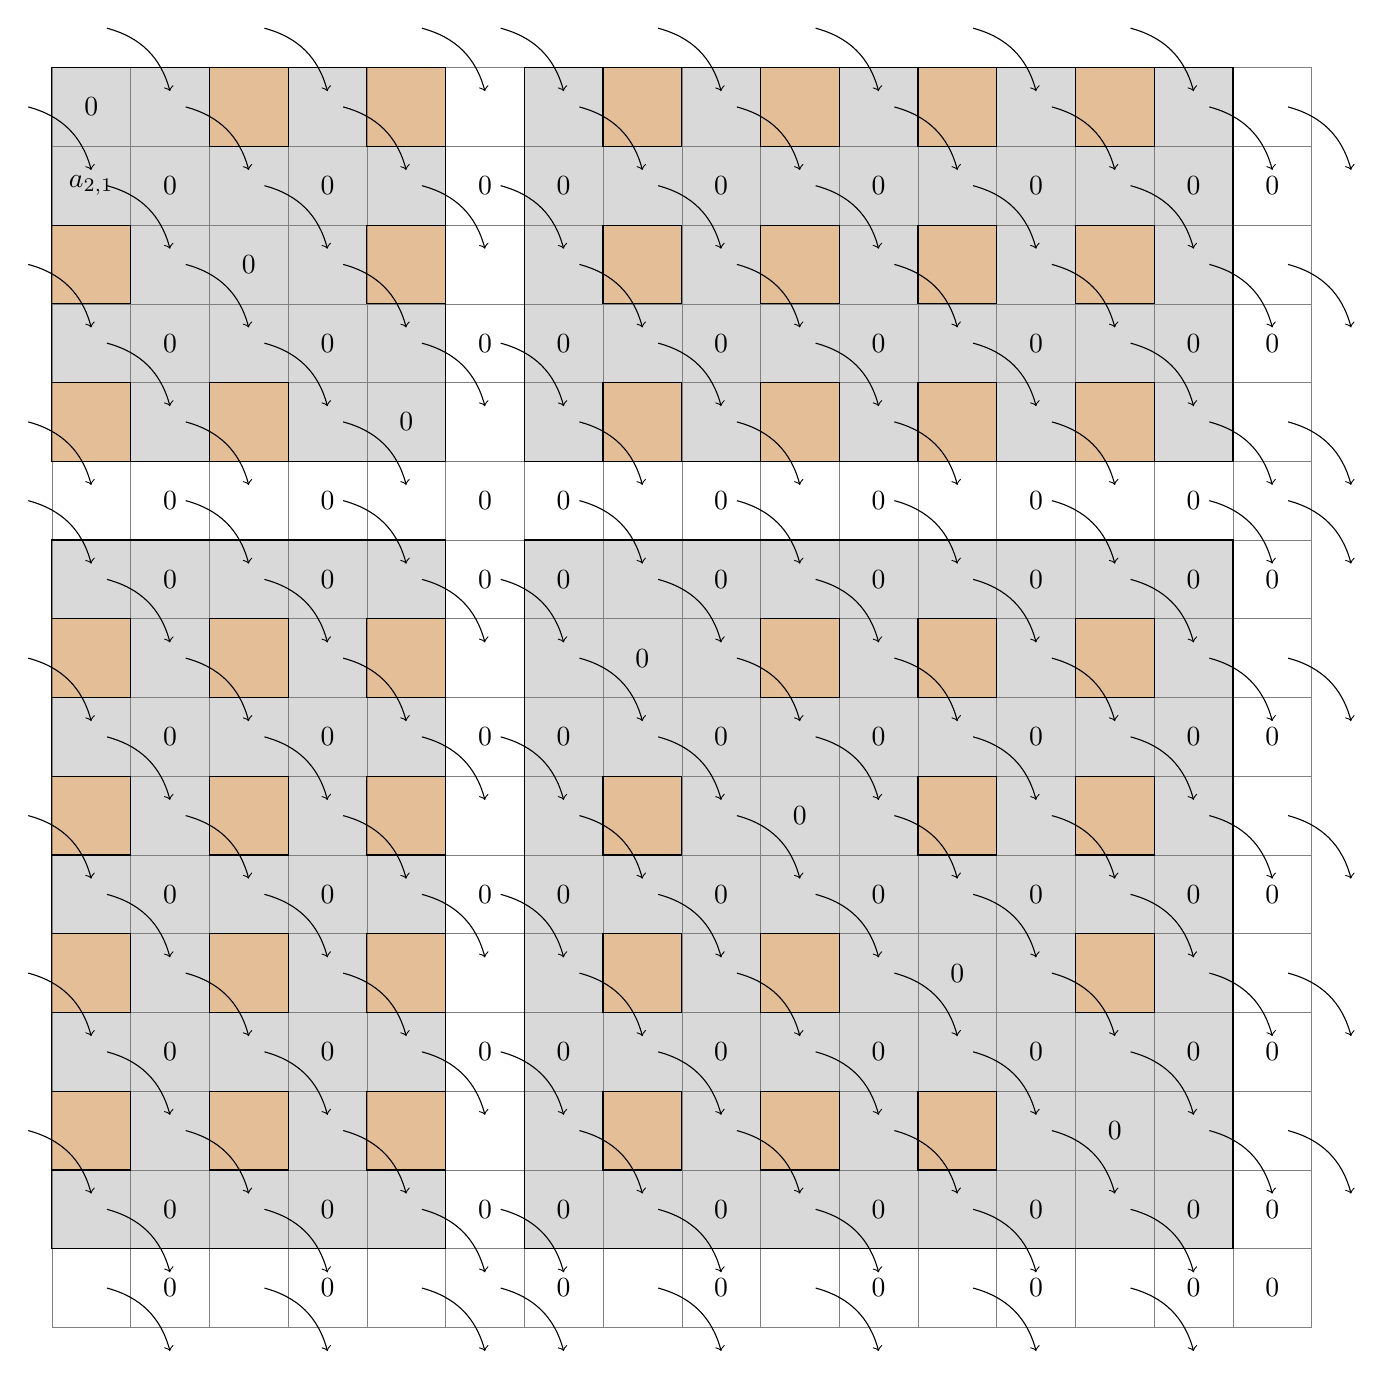
\begin{tikzpicture}
            \draw [step=1cm,gray,very thin] (0,0) grid (16,16);
            \filldraw[fill=gray, fill opacity=0.3, draw=black] (0,11) rectangle (5,16);
            \filldraw[fill=gray, fill opacity=0.3, draw=black] (6,1) rectangle (15,10);
            \filldraw[fill=gray, fill opacity=0.3, draw=black] (0,1) rectangle (5,10);
            \filldraw[fill=gray, fill opacity=0.3, draw=black] (6,11) rectangle (15,16);
            \node at (0.5,15.5){0};

            \node at (1.5,14.5){0};
            \node at (1.5,12.5){0};
            \node at (1.5,10.5){0};
            \node at (1.5,9.5){0};
            \node at (1.5,7.5){0};
            \node at (1.5,5.5){0};
            \node at (1.5,3.5){0};
            \node at (1.5,1.5){0};
            \node at (1.5,0.5){0};

            \node at (3.5,14.5){0};
            \node at (3.5,12.5){0};
            \node at (3.5,10.5){0};
            \node at (3.5,9.5){0};
            \node at (3.5,7.5){0};
            \node at (3.5,5.5){0};
            \node at (3.5,3.5){0};
            \node at (3.5,1.5){0};
            \node at (3.5,0.5){0};

            \node at (5.5,14.5){0};
            \node at (5.5,12.5){0};
            \node at (5.5,10.5){0};
            \node at (5.5,9.5){0};
            \node at (5.5,7.5){0};
            \node at (5.5,5.5){0};
            \node at (5.5,3.5){0};
            \node at (5.5,1.5){0};

            \node at (6.5,14.5){0};
            \node at (6.5,12.5){0};
            \node at (6.5,10.5){0};
            \node at (6.5,9.5){0};
            \node at (6.5,7.5){0};
            \node at (6.5,5.5){0};
            \node at (6.5,3.5){0};
            \node at (6.5,1.5){0};
            \node at (6.5,0.5){0};

            \node at (8.5,14.5){0};
            \node at (8.5,12.5){0};
            \node at (8.5,10.5){0};
            \node at (8.5,9.5){0};
            \node at (8.5,7.5){0};
            \node at (8.5,5.5){0};
            \node at (8.5,3.5){0};
            \node at (8.5,1.5){0};
            \node at (8.5,0.5){0};

            \node at (10.5,14.5){0};
            \node at (10.5,12.5){0};
            \node at (10.5,10.5){0};
            \node at (10.5,9.5){0};
            \node at (10.5,7.5){0};
            \node at (10.5,5.5){0};
            \node at (10.5,3.5){0};
            \node at (10.5,1.5){0};
            \node at (10.5,0.5){0};

            \node at (12.5,14.5){0};
            \node at (12.5,12.5){0};
            \node at (12.5,10.5){0};
            \node at (12.5,9.5){0};
            \node at (12.5,7.5){0};
            \node at (12.5,5.5){0};
            \node at (12.5,3.5){0};
            \node at (12.5,1.5){0};
            \node at (12.5,0.5){0};

            \node at (14.5,14.5){0};
            \node at (14.5,12.5){0};
            \node at (14.5,10.5){0};
            \node at (14.5,9.5){0};
            \node at (14.5,7.5){0};
            \node at (14.5,5.5){0};
            \node at (14.5,3.5){0};
            \node at (14.5,1.5){0};
            \node at (14.5,0.5){0};

            \node at (15.5,14.5){0};
            \node at (15.5,12.5){0};
            \node at (15.5,9.5){0};
            \node at (15.5,7.5){0};
            \node at (15.5,5.5){0};
            \node at (15.5,3.5){0};
            \node at (15.5,1.5){0};
            \node at (15.5,0.5){0};

            \node at (2.5,13.5){0};
            \node at (4.5,11.5){0};
            \node at (7.5,8.5){0};
            \node at (9.5,6.5){0};
            \node at (11.5,4.5){0};
            \node at (13.5,2.5){0};

            \filldraw[fill=orange, fill opacity=0.3, draw=black] (0,13) rectangle (1,14);
            \filldraw[fill=orange, fill opacity=0.3, draw=black] (0,11) rectangle (1,12);

            \filldraw[fill=orange, fill opacity=0.3, draw=black] (2,11) rectangle (3,12);

            \filldraw[fill=orange, fill opacity=0.3, draw=black] (2,15) rectangle (3,16);
            \filldraw[fill=orange, fill opacity=0.3, draw=black] (4,15) rectangle (5,16);

            \filldraw[fill=orange, fill opacity=0.3, draw=black] (4,13) rectangle (5,14);


            \filldraw[fill=orange, fill opacity=0.3, draw=black] (0,2) rectangle (1,3);
            \filldraw[fill=orange, fill opacity=0.3, draw=black] (2,2) rectangle (3,3);
            \filldraw[fill=orange, fill opacity=0.3, draw=black] (4,2) rectangle (5,3);

            \filldraw[fill=orange, fill opacity=0.3, draw=black] (0,4) rectangle (1,5);
            \filldraw[fill=orange, fill opacity=0.3, draw=black] (2,4) rectangle (3,5);
            \filldraw[fill=orange, fill opacity=0.3, draw=black] (4,4) rectangle (5,5);

            \filldraw[fill=orange, fill opacity=0.3, draw=black] (0,6) rectangle (1,7);
            \filldraw[fill=orange, fill opacity=0.3, draw=black] (2,6) rectangle (3,7);
            \filldraw[fill=orange, fill opacity=0.3, draw=black] (4,6) rectangle (5,7);

            \filldraw[fill=orange, fill opacity=0.3, draw=black] (0,8) rectangle (1,9);
            \filldraw[fill=orange, fill opacity=0.3, draw=black] (2,8) rectangle (3,9);
            \filldraw[fill=orange, fill opacity=0.3, draw=black] (4,8) rectangle (5,9);


            \filldraw[fill=orange, fill opacity=0.3, draw=black] (7,11) rectangle (8,12);
            \filldraw[fill=orange, fill opacity=0.3, draw=black] (7,13) rectangle (8,14);
            \filldraw[fill=orange, fill opacity=0.3, draw=black] (7,15) rectangle (8,16);

            \filldraw[fill=orange, fill opacity=0.3, draw=black] (9,11) rectangle (10,12);
            \filldraw[fill=orange, fill opacity=0.3, draw=black] (9,13) rectangle (10,14);
            \filldraw[fill=orange, fill opacity=0.3, draw=black] (9,15) rectangle (10,16);

            \filldraw[fill=orange, fill opacity=0.3, draw=black] (11,11) rectangle (12,12);
            \filldraw[fill=orange, fill opacity=0.3, draw=black] (11,13) rectangle (12,14);
            \filldraw[fill=orange, fill opacity=0.3, draw=black] (11,15) rectangle (12,16);

            \filldraw[fill=orange, fill opacity=0.3, draw=black] (13,11) rectangle (14,12);
            \filldraw[fill=orange, fill opacity=0.3, draw=black] (13,13) rectangle (14,14);
            \filldraw[fill=orange, fill opacity=0.3, draw=black] (13,15) rectangle (14,16);

            
            \filldraw[fill=orange, fill opacity=0.3, draw=black] (11,2) rectangle (12,3);

            \filldraw[fill=orange, fill opacity=0.3, draw=black] (9,2) rectangle (10,3);
            \filldraw[fill=orange, fill opacity=0.3, draw=black] (9,4) rectangle (10,5);
            
            \filldraw[fill=orange, fill opacity=0.3, draw=black] (7,2) rectangle (8,3);
            \filldraw[fill=orange, fill opacity=0.3, draw=black] (7,4) rectangle (8,5);
            \filldraw[fill=orange, fill opacity=0.3, draw=black] (7,6) rectangle (8,7);
            
            
            \filldraw[fill=orange, fill opacity=0.3, draw=black] (13,4) rectangle (14,5);
            
            \filldraw[fill=orange, fill opacity=0.3, draw=black] (13,6) rectangle (14,7);
            \filldraw[fill=orange, fill opacity=0.3, draw=black] (11,6) rectangle (12,7);
            
            \filldraw[fill=orange, fill opacity=0.3, draw=black] (13,8) rectangle (14,9);
            \filldraw[fill=orange, fill opacity=0.3, draw=black] (11,8) rectangle (12,9);
            \filldraw[fill=orange, fill opacity=0.3, draw=black] (9,8) rectangle (10,9);

            \draw[->] (-0.3,15.5) to[bend left] (0.5,14.7);
            \draw[->] (-0.3,13.5) to[bend left] (0.5,12.7);
            \draw[->] (-0.3,11.5) to[bend left] (0.5,10.7);
            \draw[->] (-0.3,10.5) to[bend left] (0.5,9.7);
            \draw[->] (-0.3,8.5) to[bend left] (0.5,7.7);
            \draw[->] (-0.3,6.5) to[bend left] (0.5,5.7);
            \draw[->] (-0.3,4.5) to[bend left] (0.5,3.7);
            \draw[->] (-0.3,2.5) to[bend left] (0.5,1.7);

            \draw[->] (0.7,16.5) to[bend left] (1.5,15.7);
            \draw[->] (0.7,14.5) to[bend left] (1.5,13.7);
            \draw[->] (0.7,12.5) to[bend left] (1.5,11.7);
            \draw[->] (0.7,9.5) to[bend left] (1.5,8.7);
            \draw[->] (0.7,7.5) to[bend left] (1.5,6.7);
            \draw[->] (0.7,5.5) to[bend left] (1.5,4.7);
            \draw[->] (0.7,3.5) to[bend left] (1.5,2.7);
            \draw[->] (0.7,1.5) to[bend left] (1.5,0.7);
            \draw[->] (0.7,0.5) to[bend left] (1.5,-0.3);

            \draw[->] (1.7,15.5) to[bend left] (2.5,14.7);
            \draw[->] (1.7,13.5) to[bend left] (2.5,12.7);
            \draw[->] (1.7,11.5) to[bend left] (2.5,10.7);
            \draw[->] (1.7,10.5) to[bend left] (2.5,9.7);
            \draw[->] (1.7,8.5) to[bend left] (2.5,7.7);
            \draw[->] (1.7,6.5) to[bend left] (2.5,5.7);
            \draw[->] (1.7,4.5) to[bend left] (2.5,3.7);
            \draw[->] (1.7,2.5) to[bend left] (2.5,1.7);

            \draw[->] (2.7,16.5) to[bend left] (3.5,15.7);
            \draw[->] (2.7,14.5) to[bend left] (3.5,13.7);
            \draw[->] (2.7,12.5) to[bend left] (3.5,11.7);
            \draw[->] (2.7,9.5) to[bend left] (3.5,8.7);
            \draw[->] (2.7,7.5) to[bend left] (3.5,6.7);
            \draw[->] (2.7,5.5) to[bend left] (3.5,4.7);
            \draw[->] (2.7,3.5) to[bend left] (3.5,2.7);
            \draw[->] (2.7,1.5) to[bend left] (3.5,0.7);
            \draw[->] (2.7,0.5) to[bend left] (3.5,-0.3);

            \draw[->] (3.7,15.5) to[bend left] (4.5,14.7);
            \draw[->] (3.7,13.5) to[bend left] (4.5,12.7);
            \draw[->] (3.7,11.5) to[bend left] (4.5,10.7);
            \draw[->] (3.7,10.5) to[bend left] (4.5,9.7);
            \draw[->] (3.7,8.5) to[bend left] (4.5,7.7);
            \draw[->] (3.7,6.5) to[bend left] (4.5,5.7);
            \draw[->] (3.7,4.5) to[bend left] (4.5,3.7);
            \draw[->] (3.7,2.5) to[bend left] (4.5,1.7);

            \draw[->] (4.7,16.5) to[bend left] (5.5,15.7);
            \draw[->] (4.7,14.5) to[bend left] (5.5,13.7);
            \draw[->] (4.7,12.5) to[bend left] (5.5,11.7);
            \draw[->] (4.7,9.5) to[bend left] (5.5,8.7);
            \draw[->] (4.7,7.5) to[bend left] (5.5,6.7);
            \draw[->] (4.7,5.5) to[bend left] (5.5,4.7);
            \draw[->] (4.7,3.5) to[bend left] (5.5,2.7);
            \draw[->] (4.7,1.5) to[bend left] (5.5,0.7);
            \draw[->] (4.7,0.5) to[bend left] (5.5,-0.3);


            \draw[->] (5.7,16.5) to[bend left] (6.5,15.7);
            \draw[->] (5.7,14.5) to[bend left] (6.5,13.7);
            \draw[->] (5.7,12.5) to[bend left] (6.5,11.7);
            \draw[->] (5.7,9.5) to[bend left] (6.5,8.7);
            \draw[->] (5.7,7.5) to[bend left] (6.5,6.7);
            \draw[->] (5.7,5.5) to[bend left] (6.5,4.7);
            \draw[->] (5.7,3.5) to[bend left] (6.5,2.7);
            \draw[->] (5.7,1.5) to[bend left] (6.5,0.7);
            \draw[->] (5.7,0.5) to[bend left] (6.5,-0.3);

            
            \draw[->] (6.7,15.5) to[bend left] (7.5,14.7);
            \draw[->] (6.7,13.5) to[bend left] (7.5,12.7);
            \draw[->] (6.7,11.5) to[bend left] (7.5,10.7);
            \draw[->] (6.7,10.5) to[bend left] (7.5,9.7);
            \draw[->] (6.7,8.5) to[bend left] (7.5,7.7);
            \draw[->] (6.7,6.5) to[bend left] (7.5,5.7);
            \draw[->] (6.7,4.5) to[bend left] (7.5,3.7);
            \draw[->] (6.7,2.5) to[bend left] (7.5,1.7);

            
            \draw[->] (7.7,16.5) to[bend left] (8.5,15.7);
            \draw[->] (7.7,14.5) to[bend left] (8.5,13.7);
            \draw[->] (7.7,12.5) to[bend left] (8.5,11.7);
            \draw[->] (7.7,9.5) to[bend left] (8.5,8.7);
            \draw[->] (7.7,7.5) to[bend left] (8.5,6.7);
            \draw[->] (7.7,5.5) to[bend left] (8.5,4.7);
            \draw[->] (7.7,3.5) to[bend left] (8.5,2.7);
            \draw[->] (7.7,1.5) to[bend left] (8.5,0.7);
            \draw[->] (7.7,0.5) to[bend left] (8.5,-0.3);

            \draw[->] (8.7,15.5) to[bend left] (9.5,14.7);
            \draw[->] (8.7,13.5) to[bend left] (9.5,12.7);
            \draw[->] (8.7,11.5) to[bend left] (9.5,10.7);
            \draw[->] (8.7,10.5) to[bend left] (9.5,9.7);
            \draw[->] (8.7,8.5) to[bend left] (9.5,7.7);
            \draw[->] (8.7,6.5) to[bend left] (9.5,5.7);
            \draw[->] (8.7,4.5) to[bend left] (9.5,3.7);
            \draw[->] (8.7,2.5) to[bend left] (9.5,1.7);

            \draw[->] (9.7,16.5) to[bend left] (10.5,15.7);
            \draw[->] (9.7,14.5) to[bend left] (10.5,13.7);
            \draw[->] (9.7,12.5) to[bend left] (10.5,11.7);
            \draw[->] (9.7,9.5) to[bend left] (10.5,8.7);
            \draw[->] (9.7,7.5) to[bend left] (10.5,6.7);
            \draw[->] (9.7,5.5) to[bend left] (10.5,4.7);
            \draw[->] (9.7,3.5) to[bend left] (10.5,2.7);
            \draw[->] (9.7,1.5) to[bend left] (10.5,0.7);
            \draw[->] (9.7,0.5) to[bend left] (10.5,-0.3);

            \draw[->] (10.7,15.5) to[bend left] (11.5,14.7);
            \draw[->] (10.7,13.5) to[bend left] (11.5,12.7);
            \draw[->] (10.7,11.5) to[bend left] (11.5,10.7);
            \draw[->] (10.7,10.5) to[bend left] (11.5,9.7);
            \draw[->] (10.7,8.5) to[bend left] (11.5,7.7);
            \draw[->] (10.7,6.5) to[bend left] (11.5,5.7);
            \draw[->] (10.7,4.5) to[bend left] (11.5,3.7);
            \draw[->] (10.7,2.5) to[bend left] (11.5,1.7);

            \draw[->] (11.7,16.5) to[bend left] (12.5,15.7);
            \draw[->] (11.7,14.5) to[bend left] (12.5,13.7);
            \draw[->] (11.7,12.5) to[bend left] (12.5,11.7);
            \draw[->] (11.7,9.5) to[bend left] (12.5,8.7);
            \draw[->] (11.7,7.5) to[bend left] (12.5,6.7);
            \draw[->] (11.7,5.5) to[bend left] (12.5,4.7);
            \draw[->] (11.7,3.5) to[bend left] (12.5,2.7);
            \draw[->] (11.7,1.5) to[bend left] (12.5,0.7);
            \draw[->] (11.7,0.5) to[bend left] (12.5,-0.3);

            \draw[->] (12.7,15.5) to[bend left] (13.5,14.7);
            \draw[->] (12.7,13.5) to[bend left] (13.5,12.7);
            \draw[->] (12.7,11.5) to[bend left] (13.5,10.7);
            \draw[->] (12.7,10.5) to[bend left] (13.5,9.7);
            \draw[->] (12.7,8.5) to[bend left] (13.5,7.7);
            \draw[->] (12.7,6.5) to[bend left] (13.5,5.7);
            \draw[->] (12.7,4.5) to[bend left] (13.5,3.7);
            \draw[->] (12.7,2.5) to[bend left] (13.5,1.7);

            \draw[->] (13.7,16.5) to[bend left] (14.5,15.7);
            \draw[->] (13.7,14.5) to[bend left] (14.5,13.7);
            \draw[->] (13.7,12.5) to[bend left] (14.5,11.7);
            \draw[->] (13.7,9.5) to[bend left] (14.5,8.7);
            \draw[->] (13.7,7.5) to[bend left] (14.5,6.7);
            \draw[->] (13.7,5.5) to[bend left] (14.5,4.7);
            \draw[->] (13.7,3.5) to[bend left] (14.5,2.7);
            \draw[->] (13.7,1.5) to[bend left] (14.5,0.7);
            \draw[->] (13.7,0.5) to[bend left] (14.5,-0.3);

            \draw[->] (14.7,15.5) to[bend left] (15.5,14.7);
            \draw[->] (14.7,13.5) to[bend left] (15.5,12.7);
            \draw[->] (14.7,11.5) to[bend left] (15.5,10.7);
            \draw[->] (14.7,10.5) to[bend left] (15.5,9.7);
            \draw[->] (14.7,8.5) to[bend left] (15.5,7.7);
            \draw[->] (14.7,6.5) to[bend left] (15.5,5.7);
            \draw[->] (14.7,4.5) to[bend left] (15.5,3.7);
            \draw[->] (14.7,2.5) to[bend left] (15.5,1.7);

            \draw[->] (15.7,15.5) to[bend left] (16.5,14.7);
            \draw[->] (15.7,13.5) to[bend left] (16.5,12.7);
            \draw[->] (15.7,11.5) to[bend left] (16.5,10.7);
            \draw[->] (15.7,10.5) to[bend left] (16.5,9.7);
            \draw[->] (15.7,8.5) to[bend left] (16.5,7.7);
            \draw[->] (15.7,6.5) to[bend left] (16.5,5.7);
            \draw[->] (15.7,4.5) to[bend left] (16.5,3.7);
            \draw[->] (15.7,2.5) to[bend left] (16.5,1.7);

            \node at (0.5,14.5){$a_{2,1}$};
        \end{tikzpicture}
    \end{center}


\end{proof}

\end{document}
